\section{Connecting Components} \label{sc:connecting_components}
The components have been defined in the above sections and their connections and desired interactions will be described and depicted in the following section.
\par
The model and function components have a few dependencies between them. These dependencies have been converted to connections in a way that gives the most cohesion in the system and the lowest coupling. On top of these criteria, an intuitive design and connection between the components have been striven towards.
\par
The connection between the \textit{Asset}, \textit{Tag}, and \textit{Department} classes and the \textit{Repository} strategy is an aggregation. This is because the concrete strategies handle objects of their designated type as a collection and will contain multiple instances of the class.
\par
The user interface component has a connection to the \textit{Session} class in the function component to ensure that the user can only access the functions belonging to the session. The connection exists as a call, because the relation's only purpose is to ensure that the user's information is available to the system.
\par
The user interface component is also connected with a call relation to the \textit{ExportHandler} class, as the user, if they have admin access, simply calls the function within the \textit{ExportHandler} to export a list of assets.
\par
The \textit{FieldController} contains the functionality to add fields to objects that allow it. The user, if they have admin access, should have access to this functionality and therefore, the user interface has a call relation to the \textit{FieldController} in the function component.
\par
The repository strategy has a connection to the database, to save the different models in the database. This is simply a call relation, as the repositories just need to call the operations on the database.
\\\\
The above descriptions has described the connections between the model and function components. The decisions reasoned above have resulted in the following component diagram.

\begin{figure}[H]
    \centering
    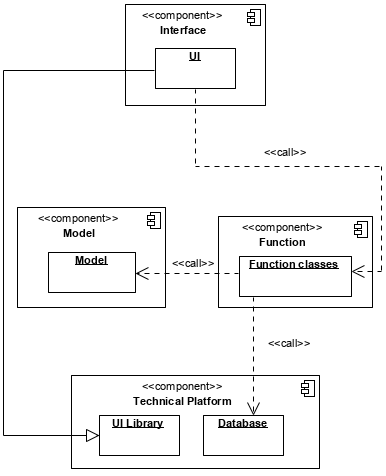
\includegraphics[width=0.8\textwidth]{figures/ComponentDiagrams/ComponentDesignOverview.png}
    \caption{Illustration of the component design of the system}
    \label{fig:FinalComponentDesign}
\end{figure}

\todo[inline]{Actual connection of components diagram}

With the component design constructed and illustrated, the UI can be designed. The UI design will build on the component design and the results from the previous analysis.